\section{A Cascade Model of Standard PSO}
\label{sec:sys_model}

In this paper, we model the behavior of the PSO algorithm as a \emph{cascade system}.
This enables analysis of PSO with stochastic factors preserved and without the stagnation assumption.
As shown in Figure \ref{fig:sys_flow}, this system is comprised of two components that form a
cascade system structure.
These two components are the 
\emph{input update component} for the global best ($ x^{G}_{i}(k) $) and the personal best ($ x^{P}_{i}(k) $), and the 
\emph{position update component} for particle position ($ x_{i}(k+1) $), which depends on the inputs $ x^{G}_{i}(k) $ and $ x^{P}_{i}(k) $ as well as the last position $ x_{i}(k) $ and the swarm topology.

\begin{figure}
\centering
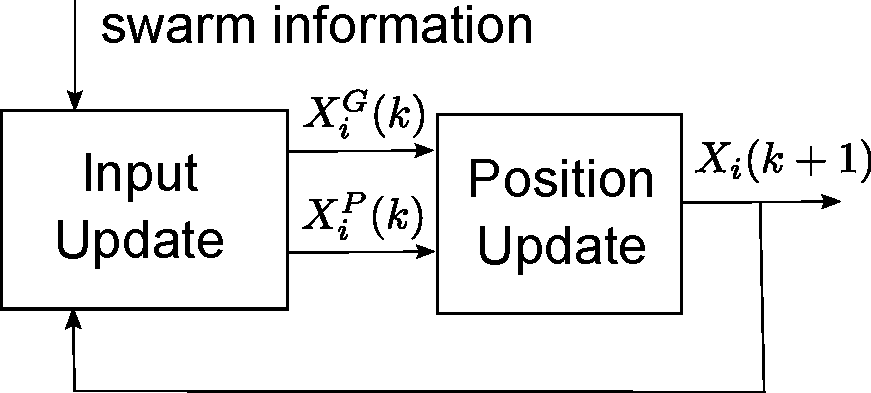
\includegraphics[width=0.5\textwidth]{sys_flow.pdf}
\caption{System structure of PSO}
\label{fig:sys_flow}
\end{figure}

The properties of this system can be analyzed using the input-to-state stability of the position update component and the input update component. 
Given an input-to-state stable position update component, we will see that the convergence of $ x_{i}(k) $ depends on bounds on $ x^{G}_{i}(k) $ and $ x^{P}_{i}(k) $.

%PSO is designed to strike an effective balance between \emph{exploring} and \emph{exploiting} a fitness landscape.
%A bound on a particle's state is an indicator of the nature of that balance.
%When this bound is large the particle is exploring.
%However, as a particle finishes exploring and reach stagnation, a particle's position should converge.
%
%Input-to-state stability implies that the state of the system is bounded in a range determined by the bounds on the input.
%Before stagnation, when the personal best and global best values have not converged, we can expect only looser bounds on the particle state.
%These looser bounds reflect both what is know about the input and the what is know about the update process itself.
%
%
%We call the bounds on the global best and personal best the ``exploit radius'' and the bounds on the particle's position a ``explore radius''.
%The ratio of the explore radius to the exploit radius is determined by the parameters of the position update component.
%However, if the personal best and global best converge to an estimated optimal position, the exploit radius falls to zero and the explore radius declines to a bound.
%
%\begin{figure}
%\centering
%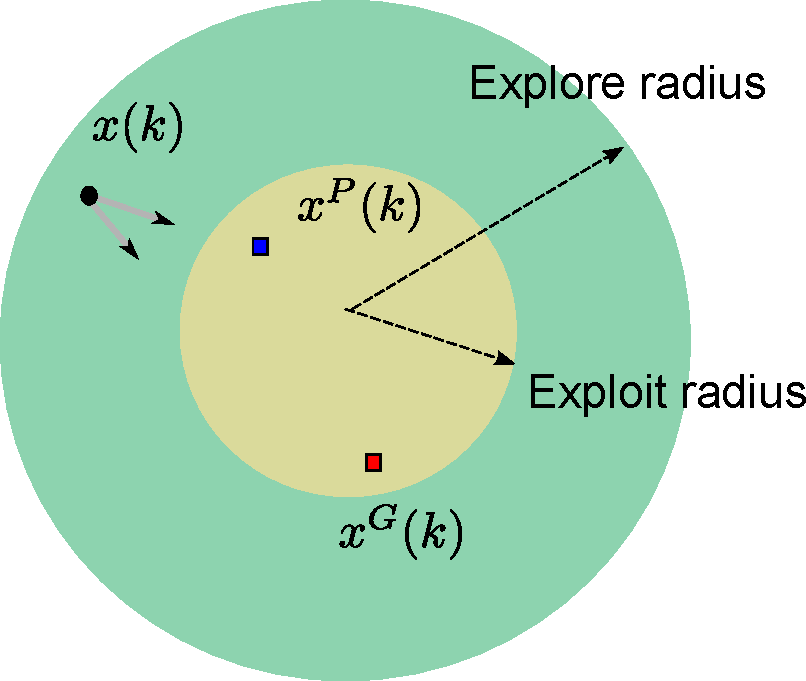
\includegraphics[width=0.4\textwidth]{./explore_and_exploit}
%\caption{Exploration and exploitation.}
%\label{fig:explore_and_exploit}
%\end{figure}

In our analysis of the PSO algorithm, we seek to understand how the particles converge to some position $ x^{*} $, which is intended (not guaranteed) by the algorithm to be the optimal position.

Without loss of generality, we look at a one-dimension particle and extract the linear form of the position update component.
\begin{equation}
\label{eq:pso_up_linalg_simp}
X(k+1) = A(k) X(k) + B(k) U(k)
\end{equation}
with
$ A(k) = \begin{bmatrix}
\chi & - \chi \phi^{G} u^{G}(k) - \chi \phi^{P} u^{P}(k)
\\ 
\chi & 1 - \chi \phi^{G} u^{G}(k) - \chi \phi^{P} u^{P}(k)
\end{bmatrix} $
and
$ B(k) = \begin{bmatrix}
\chi \phi^{G} u^{G}(k) & \chi \phi^{P} u^{P}(k)
\\ 
\chi \phi^{G} u^{G}(k) & \chi \phi^{P} u^{P}(k)
\end{bmatrix} $.

The system state is $ X(k) = [ v(k), x(k) - x^{*} ]^{T} $, and the system input is $ U(k) = [ x^{G}(k) - x^{*} , x^{P}(k) - x^{*} ]^{T} $
\footnote{$ x^{*} $ means an equilibrium point to the system.
In PSO, it can be a local optimum, a global optimum, or an estimated optimum.
We use it as a reference point to check the bounds.}
.
The convergence of this model means that $ v(k) \rightarrow 0 $ and $ x(k) \rightarrow x^{*} $.

